\documentclass{standalone}
\usepackage{tikz}
\usepackage{ctex,siunitx}
\setCJKmainfont{Noto Serif CJK SC}
\usepackage{tkz-euclide}
\usepackage{amsmath}
\usetikzlibrary{patterns, calc}
\usetikzlibrary {decorations.pathmorphing, decorations.pathreplacing, decorations.shapes,}
\begin{document}
\small
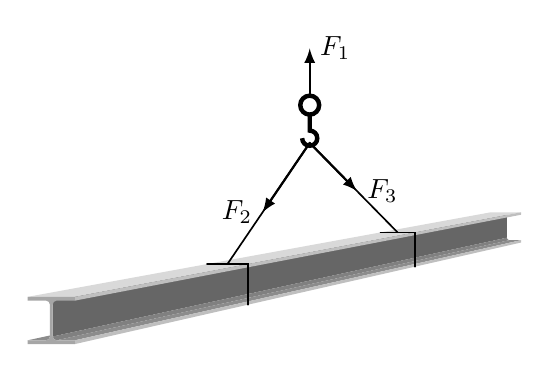
\begin{tikzpicture}[>=latex,scale=1.2]
  % \useasboundingbox(-0.25,-0.25)rectangle(4,3);
  \fill[darkgray!80]( 2.086,-1.003)--(-2.720,-2.049)--(-2.720,-1.648)--( 2.086,-0.753)--cycle;
  \fill[gray](-2.680,-2.089)..controls(-2.700,-2.089)and(-2.720,-2.069)..(-2.720,-2.049)--( 2.086,-1.003)..controls( 2.086,-1.016)and( 2.099,-1.029)..( 2.112,-1.029)--cycle;
  \fill[gray!90]( 2.237,-1.029)--(-2.485,-2.089)--(-2.680,-2.089)--( 2.112,-1.029)--cycle
  (-2.750,-2.049)..controls(-2.750,-2.069)and(-2.770,-2.089)..(-2.790,-2.089)--(-2.985,-2.089)--(-2.750,-2.038)--cycle;
  \fill[gray!30]
  (-2.985,-1.629)--( 1.917,-0.734)--( 2.237,-0.734)--(-2.485,-1.629)--cycle;
  \fill[lightgray](-2.485,-2.129)--( 2.237,-1.054)--( 2.237,-1.029)--(-2.485,-2.089)--cycle
  (-2.485,-1.669)--( 2.237,-0.760)--( 2.237,-0.734)--(-2.485,-1.629)--cycle;
  \fill[gray!70](-2.680,-2.089)..controls(-2.700,-2.089)and(-2.720,-2.069)..(-2.720,-2.049)--(-2.720,-1.709)..controls(-2.720,-1.689)and(-2.700,-1.669)..(-2.680,-1.669)--(-2.485,-1.669)--(-2.485,-1.629)--(-2.985,-1.629)--(-2.985,-1.669)--(-2.790,-1.669)..controls(-2.770,-1.669)and(-2.750,-1.689)..(-2.750,-1.709)--(-2.750,-2.049)..controls(-2.750,-2.069)and(-2.770,-2.089)..(-2.790,-2.089)--(-2.985,-2.089)--(-2.985,-2.129)--(-2.485,-2.129)--(-2.485,-2.089)--cycle;
  \draw[line cap=round,semithick](-1.0863,-1.2826)--(-0.6560,-1.2826)--(-0.6560,-1.7129);
  \draw[line cap=round,semithick]( 0.7492,-0.9475)--(1.1120,-0.9475)--(1.1120,-1.3104);
  \draw[semithick](-0.8711,-1.2826)--(0,0)--(0.9306,-0.9475);
  \draw[thick,->](0,0)--(-0.5,-0.736)node[left]{$F_2$};
  \draw[thick,->](0,0)--(0.5,-0.509)node[right]{$F_3$};
  \draw[ultra thick](-0.08,0.05)arc(-180:90:0.08)--++(0,0.15)(0,0.4)circle(0.1);
  \draw[thick,->](0,0.5)--(0,1.0)node[right]{$F_1$};
\end{tikzpicture}
\end{document}